% Options for packages loaded elsewhere
\PassOptionsToPackage{unicode}{hyperref}
\PassOptionsToPackage{hyphens}{url}
%
\documentclass[
  man,mask,floatsintext]{apa7}
\usepackage{amsmath,amssymb}
\usepackage{iftex}
\ifPDFTeX
  \usepackage[T1]{fontenc}
  \usepackage[utf8]{inputenc}
  \usepackage{textcomp} % provide euro and other symbols
\else % if luatex or xetex
  \usepackage{unicode-math} % this also loads fontspec
  \defaultfontfeatures{Scale=MatchLowercase}
  \defaultfontfeatures[\rmfamily]{Ligatures=TeX,Scale=1}
\fi
\usepackage{lmodern}
\ifPDFTeX\else
  % xetex/luatex font selection
\fi
% Use upquote if available, for straight quotes in verbatim environments
\IfFileExists{upquote.sty}{\usepackage{upquote}}{}
\IfFileExists{microtype.sty}{% use microtype if available
  \usepackage[]{microtype}
  \UseMicrotypeSet[protrusion]{basicmath} % disable protrusion for tt fonts
}{}
\makeatletter
\@ifundefined{KOMAClassName}{% if non-KOMA class
  \IfFileExists{parskip.sty}{%
    \usepackage{parskip}
  }{% else
    \setlength{\parindent}{0pt}
    \setlength{\parskip}{6pt plus 2pt minus 1pt}}
}{% if KOMA class
  \KOMAoptions{parskip=half}}
\makeatother
\usepackage{xcolor}
\usepackage{graphicx}
\makeatletter
\def\maxwidth{\ifdim\Gin@nat@width>\linewidth\linewidth\else\Gin@nat@width\fi}
\def\maxheight{\ifdim\Gin@nat@height>\textheight\textheight\else\Gin@nat@height\fi}
\makeatother
% Scale images if necessary, so that they will not overflow the page
% margins by default, and it is still possible to overwrite the defaults
% using explicit options in \includegraphics[width, height, ...]{}
\setkeys{Gin}{width=\maxwidth,height=\maxheight,keepaspectratio}
% Set default figure placement to htbp
\makeatletter
\def\fps@figure{htbp}
\makeatother
\setlength{\emergencystretch}{3em} % prevent overfull lines
\providecommand{\tightlist}{%
  \setlength{\itemsep}{0pt}\setlength{\parskip}{0pt}}
\setcounter{secnumdepth}{-\maxdimen} % remove section numbering
% Make \paragraph and \subparagraph free-standing
\ifx\paragraph\undefined\else
  \let\oldparagraph\paragraph
  \renewcommand{\paragraph}[1]{\oldparagraph{#1}\mbox{}}
\fi
\ifx\subparagraph\undefined\else
  \let\oldsubparagraph\subparagraph
  \renewcommand{\subparagraph}[1]{\oldsubparagraph{#1}\mbox{}}
\fi
% definitions for citeproc citations
\NewDocumentCommand\citeproctext{}{}
\NewDocumentCommand\citeproc{mm}{%
  \begingroup\def\citeproctext{#2}\cite{#1}\endgroup}
\makeatletter
 % allow citations to break across lines
 \let\@cite@ofmt\@firstofone
 % avoid brackets around text for \cite:
 \def\@biblabel#1{}
 \def\@cite#1#2{{#1\if@tempswa , #2\fi}}
\makeatother
\newlength{\cslhangindent}
\setlength{\cslhangindent}{1.5em}
\newlength{\csllabelwidth}
\setlength{\csllabelwidth}{3em}
\newenvironment{CSLReferences}[2] % #1 hanging-indent, #2 entry-spacing
 {\begin{list}{}{%
  \setlength{\itemindent}{0pt}
  \setlength{\leftmargin}{0pt}
  \setlength{\parsep}{0pt}
  % turn on hanging indent if param 1 is 1
  \ifodd #1
   \setlength{\leftmargin}{\cslhangindent}
   \setlength{\itemindent}{-1\cslhangindent}
  \fi
  % set entry spacing
  \setlength{\itemsep}{#2\baselineskip}}}
 {\end{list}}
\usepackage{calc}
\newcommand{\CSLBlock}[1]{\hfill\break\parbox[t]{\linewidth}{\strut\ignorespaces#1\strut}}
\newcommand{\CSLLeftMargin}[1]{\parbox[t]{\csllabelwidth}{\strut#1\strut}}
\newcommand{\CSLRightInline}[1]{\parbox[t]{\linewidth - \csllabelwidth}{\strut#1\strut}}
\newcommand{\CSLIndent}[1]{\hspace{\cslhangindent}#1}
\ifLuaTeX
\usepackage[bidi=basic]{babel}
\else
\usepackage[bidi=default]{babel}
\fi
\babelprovide[main,import]{english}
% get rid of language-specific shorthands (see #6817):
\let\LanguageShortHands\languageshorthands
\def\languageshorthands#1{}
% Manuscript styling
\usepackage{upgreek}
\captionsetup{font=singlespacing,justification=justified}

% Table formatting
\usepackage{longtable}
\usepackage{lscape}
% \usepackage[counterclockwise]{rotating}   % Landscape page setup for large tables
\usepackage{multirow}		% Table styling
\usepackage{tabularx}		% Control Column width
\usepackage[flushleft]{threeparttable}	% Allows for three part tables with a specified notes section
\usepackage{threeparttablex}            % Lets threeparttable work with longtable

% Create new environments so endfloat can handle them
% \newenvironment{ltable}
%   {\begin{landscape}\centering\begin{threeparttable}}
%   {\end{threeparttable}\end{landscape}}
\newenvironment{lltable}{\begin{landscape}\centering\begin{ThreePartTable}}{\end{ThreePartTable}\end{landscape}}

% Enables adjusting longtable caption width to table width
% Solution found at http://golatex.de/longtable-mit-caption-so-breit-wie-die-tabelle-t15767.html
\makeatletter
\newcommand\LastLTentrywidth{1em}
\newlength\longtablewidth
\setlength{\longtablewidth}{1in}
\newcommand{\getlongtablewidth}{\begingroup \ifcsname LT@\roman{LT@tables}\endcsname \global\longtablewidth=0pt \renewcommand{\LT@entry}[2]{\global\advance\longtablewidth by ##2\relax\gdef\LastLTentrywidth{##2}}\@nameuse{LT@\roman{LT@tables}} \fi \endgroup}

% \setlength{\parindent}{0.5in}
% \setlength{\parskip}{0pt plus 0pt minus 0pt}

% Overwrite redefinition of paragraph and subparagraph by the default LaTeX template
% See https://github.com/crsh/papaja/issues/292
\makeatletter
\renewcommand{\paragraph}{\@startsection{paragraph}{4}{\parindent}%
  {0\baselineskip \@plus 0.2ex \@minus 0.2ex}%
  {-1em}%
  {\normalfont\normalsize\bfseries\itshape\typesectitle}}

\renewcommand{\subparagraph}[1]{\@startsection{subparagraph}{5}{1em}%
  {0\baselineskip \@plus 0.2ex \@minus 0.2ex}%
  {-\z@\relax}%
  {\normalfont\normalsize\itshape\hspace{\parindent}{#1}\textit{\addperi}}{\relax}}
\makeatother

\makeatletter
\usepackage{etoolbox}
\patchcmd{\maketitle}
  {\section{\normalfont\normalsize\abstractname}}
  {\section*{\normalfont\normalsize\abstractname}}
  {}{\typeout{Failed to patch abstract.}}
\patchcmd{\maketitle}
  {\section{\protect\normalfont{\@title}}}
  {\section*{\protect\normalfont{\@title}}}
  {}{\typeout{Failed to patch title.}}
\makeatother

\usepackage{xpatch}
\makeatletter
\xapptocmd\appendix
  {\xapptocmd\section
    {\addcontentsline{toc}{section}{\appendixname\ifoneappendix\else~\theappendix\fi\\: #1}}
    {}{\InnerPatchFailed}%
  }
{}{\PatchFailed}
\keywords{COVID-19, well-being, social media, news use, panel study.}
\usepackage{csquotes}
\makeatletter
\renewcommand{\paragraph}{\@startsection{paragraph}{4}{\parindent}%
  {0\baselineskip \@plus 0.2ex \@minus 0.2ex}%
  {-1em}%
  {\normalfont\normalsize\bfseries\typesectitle}}

\renewcommand{\subparagraph}[1]{\@startsection{subparagraph}{5}{1em}%
  {0\baselineskip \@plus 0.2ex \@minus 0.2ex}%
  {-\z@\relax}%
  {\normalfont\normalsize\bfseries\itshape\hspace{\parindent}{#1}\textit{\addperi}}{\relax}}
\makeatother
\usepackage{endnotes}
\setlength{\parskip}{0em}
\raggedbottom
\note{\clearpage}
\usepackage{setspace}
\AtBeginEnvironment{tabular}{\singlespacing}
\AtBeginEnvironment{lltable}{\singlespacing}
\AtBeginEnvironment{tablenotes}{\doublespacing}
\captionsetup[table]{font={stretch=1.5}}
\captionsetup[figure]{font={stretch=1.5}}

\ifLuaTeX
  \usepackage{selnolig}  % disable illegal ligatures
\fi
\IfFileExists{bookmark.sty}{\usepackage{bookmark}}{\usepackage{hyperref}}
\IfFileExists{xurl.sty}{\usepackage{xurl}}{} % add URL line breaks if available
\urlstyle{same}
\hypersetup{
  pdftitle={Effects of COVID-19 related social media use on well-being},
  pdflang={en-EN},
  pdfkeywords={COVID-19, well-being, social media, news use, panel study.},
  hidelinks,
  pdfcreator={LaTeX via pandoc}}

\title{Effects of COVID-19 related social media use on well-being}
\author{Name blinded for review\textsuperscript{1}}
\date{}


\shorttitle{Effects of COVID-19 related social media use on well-being}

\authornote{

Correspondence concerning this article should be addressed to Name blinded for review, . E-mail:

}

\affiliation{\vspace{0.5cm}\textsuperscript{1} }

\abstract{%
In times of crisis such as the COVID-19 pandemic, citizens need to stay informed about recent political events. To this end, people increasingly use social media. However, because social media are particularly engaging, many find it hard to disconnect, especially during times of crisis. In this preregistered study, I investigate whether using social media for COVID-19 related reasons affects psychological well-being. Using data from the Austrian Corona Panel Project consisting of 3,485 participants from 34 waves, this research question was analyzed using random effects within between models, controlling for several stable and varying confounders. The results showed that COVID-19 related social media use did not meaningfully reduce well-being. Other factors such as health, income, exercise, or internal locus of control showed larger and meaningful effects.
}



\begin{document}
\maketitle

\section{Research Transparency Statement}\label{research-transparency-statement}

Conflicts of interest: The author declares no conflicts of interest. Funding: This research did not receive external funding. Artificial intelligence: Chat GPT was used for language polishing. Ethics: This research complies with the Declaration of Helsinki (2023), aside from the requirement to preregister human subjects research. Ethical review and approval was not required for the study in accordance with the local legislation and institutional requirements. The participants provided their written informed consent to participate in this study. Computational reproducibility: All analyses and the manuscript itself are completely reproducible (\url{https://XMtRA.github.io/Austrian_Corona_Panel_Project}).

Preregistration: The hypotheses, the sample, the measures, the analyses, and the inference criteria (SESOI, \emph{p}-value) were preregistered on the Open Science Framework (\url{https://osf.io/87b24/?view_only=b2289b6fec214fa88ee75a18d45c18f3}).
Because in this study data from an already existing data set was analyzed, the preregistration was done prior to accessing the data.
In some cases, it was impossible to execute the analyses as originally planned, for example because some properties of the variables only became apparent when seeing the actual data.
All changes are reported online (\url{https://xmtra.github.io/Austrian_Corona_Panel_Project/preregistration_changes.html}).
Materials: All study materials are publicly available (\url{https://xmtra.github.io/Austrian_Corona_Panel_Project/items_english.html}). Data: All primary data are publicly available (\url{https://doi.org/10.11587/28KQNS}). Analysis scripts: All analysis scripts are publicly available (\url{https://XMtRA.github.io/Austrian_Corona_Panel_Project}).

\newpage

\section{Introduction}\label{introduction}

Amidst the COVID-19 pandemic, staying informed became paramount, prompting heavy reliance on social media for updates, with use being at an all time high (Statista, 2021).
The phenomenon of ``doomscrolling'' emerged as individuals struggled to disengage from COVID-19-related news (Buchanan et al., 2021; Sharma et al., 2022), sparking concerns about its impact on mental health (Sandstrom et al., 2021).
While initial research began exploring this question (e.g., Bendau et al., 2021; Eden et al., 2020; Sewall et al., 2021), the extent of social media's influence on well-being remains largely unknown.
This study aims to assess the effects of different social media usage patterns on individual well-being using a comprehensive longitudinal dataset spanning 34 waves, offering insights into within-person causal relationships.

\subsection{Understanding Well-being and Media Use}\label{understanding-well-being-and-media-use}

This study investigates how different \emph{facets} of subjective well-being are affected by different \emph{types} and different \emph{channels} of communication (Meier \& Reinecke, 2020).
Building on the typology of subjective well-being---defined as ``referring to the various types of subjective evaluations of one's life, including both cognitive evaluations and affective
feelings'' (Diener et al., 2018, p. 3)---three different well-being facets are analyzed: life satisfaction, positive affect, and negative affect.

Social media is a broad term, encompassing subdimensions such as social networking sites (e.g., Facebook or Instagram), instant messengers (e.g., WhatsApp or Signal), or interactive video-platforms (e.g., YouTube or TikTok) (Carr \& Hayes, 2015).
Effects of social media depend on how they are used: while purposeful, active, social use is generally related to positive outcomes, passive, non-purposeful and asocial use is related to negative outcomes (Frison \& Eggermont, 2015; Verduyn et al., 2022).
In this study, I hence distinguish three types of use and five popular channels.
The types of use include posting (active use), reading (passive use), and liking and sharing (low-threshold active use) COVID-19 related content.
The five channels to be investigated are Facebook, Twitter, Instagram, WhatsApp, and YouTube, which at the time ranked among the most popular social media services in Austria.

\subsection{Social Media Effects on Well-Being}\label{social-media-effects-on-well-being}

Current literature overviews suggest that social media use on average does seem to decrease well-being (Meier \& Reinecke, 2020).
However, for most well-being outcomes, such as life satisfaction, general well-being, or loneliness, the effects are small (Meier \& Reinecke, 2020).
These small findings can be explained with the differential susceptibility of media effects model (Valkenburg \& Peter, 2013), which states that there is substantial \emph{variation} of media effects for individual users.
For example, in one study it was estimated that roughly one quarter of all users experienced negative effects, another quarter positive effects, while for the rest the effects were neutral (Beyens et al., 2021).

Why are the effects of social media use on well-being small on average?
Two prominent media effect theories argue implicitly against strong average negative effects.
First, according to mood management theory (Zillmann, 1988), using media can affect people's moods.
After some time, users implicitly learn which media help them balance their mood and affect according to their own situational needs (Zillmann, 1988).
Those media that eventually become part of one's media repertoire hence, on average, tend to be beneficial for users to regulate their mood (Marciano et al., 2022).
In conclusion, if a certain medium is used frequently, mood-management theory argues that it is likely not detrimental for well-being.

Second, while mood management theory considers media use mainly driven by implicit learning experiences, uses and gratifications theory upholds that the process is more explicit and rational (Katz et al., 1973).
Users select those media that they expect to have a desired effect, for example on mood, knowledge, or entertainment.
And social media, in general, offer several beneficial effects, explaining their ubiquitous use.
They help find relevant information, maintain and foster relationships, express one's personality, and entertain oneself (Pelletier et al., 2020).

Third, and closely related, media use affords both both positive and negative mechanisms, which differently impact well-being outcomes.
These include factors like social comparison, inspiration, social connectedness, social support, displacement of in-person activities, information management, information overload, misinformation, reputation building, romantic connection, coping resources, or emotional contagion (Clark et al., 2018; Hall \& Liu, 2022; Pelletier et al., 2020; Vanden Abeele, 2021; Verduyn et al., 2022).
Given these differential mechanisms, strong one-sided effects appear less likely than nuanced and moderate effects.

\subsection{Social Media During COVID-19}\label{social-media-during-covid-19}

If we look at COVID-19 related use more specifically, how could the various types and channels of COVID-19 related social media use affect well-being?
Several uses and gratifications exist, which help explain why people used social media frequently during the pandemic.
Despite incorrect information, social media provide a vast platform for disseminating \emph{accurate and timely information} about COVID-19 (John Hopkins University, 2023).
Social media platforms enable individuals to \emph{connect with others} who are experiencing similar challenges during the pandemic (Guazzini et al., 2022).
Many mental health organizations and professionals utilize social media to share tips, strategies, and resources for \emph{maintaining mental well-being} during the pandemic.
Social media campaigns and initiatives can promote \emph{positive COVID-19 behaviors}, such as mask-wearing, physical distancing, hand hygiene, and vaccination (Hunt et al., 2022), which ultimately benefit well-being.

On the other hand, the effects might be negative, perhaps best explained by the following five mechanisms.
Social media platforms can easily spread \emph{false or misleading information} about COVID-19 (Li et al., 2020).
Constant exposure to COVID-19-related content on social media can lead to \emph{information overload} and contribute to heightened anxiety levels (Fan \& Smith, 2021).
Discussions around COVID-19 are known for fostering negativity, with users sometimes engaging in \emph{cyberbullying and harassment}.
Social media often showcase the highlights and accomplishments of others, encouraging \emph{social comparison} (Przybylski et al., 2013).
During a pandemic, seeing posts about others' successes or seemingly perfect lives might intensify feelings of inadequacy or FOMO, especially when individuals are unable to participate in similar activities due to restrictions or personal circumstances (Sharma et al., 2022).

Echoing the theoretical rationales outlines above, empirical studies have yielded mixed results.
Some studies found negative effects, indicating that excessive social media use for COVID-19 content led to compulsive behavior and increased stress levels, particularly due to upward social comparison (Stainback et al., 2020).
Individuals who relied on social media as their primary information source reported higher levels of anxiety and depression symptoms (Bendau et al., 2021).
Doom-scrolling was associated with negative emotional experiences (Buchanan et al., 2021).
On the other hand, some studies reported positive outcomes.
Certain individuals experienced increased virtual community and social connectedness during the pandemic through social media, which contributed to their well-being (Guazzini et al., 2022).
Additionally, identification with social media networks was associated with reduced feelings of loneliness (Latikka et al., 2022).
Several studies reported mostly neutral or dual effects of social media use on well-being indicators (Eden et al., 2020; Sewall et al., 2021).

In conclusion, given these mixed empirical results, together with the observation that social media effects on well-being are very small in general, and that several plausible theoretical mechanisms exist for both positive and negative effects, I expect that COVID-19 related communication on social media should not be decidedly positive or negative.

\begin{quote}
Hypothesis: The within-person effects of all measures of COVID-19 related social media use (types: reading, liking and sharing, posting; channels: Twitter, Instagram, Facebook, YouTube, WhatsApp) on all measures of well-being indicators (positive affect, negative affect, life satisfaction)---while controlling for several stable and varying covariates such as sociodemographic variables and psychological dispositions (see below)---will be trivial.
\end{quote}

\subsection{Smallest Effect Size of Interest}\label{smallest-effect-size-of-interest}

Exploring the hypothesis entails establishing the criteria for discerning a `trivial effect size.'
To achieve this, it is necessary to define the smallest effect size of interest (SESOI) (Anvari \& Lakens, 2021).
In this context, a trivial effect should fall below the threshold set by the SESOI (detailed below).
Determining what constitutes a minimally intriguing, nontrivial effect is a matter with normative implications, making it challenging to arrive at a definitive, singular consensus.
I propose the following SESOI as a suitable reference point for this study:

\begin{quote}
SESOI: If a heavy user of COVID-19 related social media content suddenly \emph{stops} using social media altogether, this should have a \emph{noticeable} impact on their overall well-being.
\end{quote}

Put concretely, in this study COVID-19 related social media use was measured on a 5-point scale, ranging from 1 = \emph{never} to 5 = \emph{several times a day}. Thus, a change of four units in social media use (e.g., a complete stop) should correspond to a noticeable change in well-being.
According to Norman et al. (2003), people can reliably notice seven levels of change in satisfaction with health.
So if satisfaction is measured on a 7-point scale, a four unit change in social media use should result in a one unit change in life satisfaction.
Life satisfaction was measured on an 11-point scale, and affect on a 5-point scale.
Transposed to this scaling, the SESOI for life satisfaction is \emph{b} = ±.30, and for positive and negative affect \emph{b} = ±.15 (see online supplementary material).

\section{Method}\label{method}

\subsection{Sample}\label{sample}

The data come from the Austrian Corona Panel Project (Kittel et al., 2020), which is a large-scale standalone panel study, consisting of 34 waves.
The study was conducted between March 2020 and February 2023.
Between March 2020 and July 2020, the intervals between waves were weekly, until May 2022 (wave 32) monthly, and afterward after 5 months.
Each wave consists of at least 1,500 respondents.
Panel mortality (on average ca. 5 percent per wave) was compensated through a continuous re-acquisition of new participants (on average ca. 80 new respondents per wave).
The sample size was \emph{N} = 3,641, with overall 123,794 observations.

Achieved via quota sampling, the sample matched the Austrian population in terms of age, gender, region/state, municipality size, and educational level.
In order to participate in the study, the respondents needed to be Austrian residents and had to be at least 14 years of age.
All respondents needed to have access to the internet (via computer or mobile devices such as smartphones or tablets).
The average age was 40 years, 49 percent were male, 14 percent had a University degree, and 5 percent were currently unemployed.

\subsection{Data Analysis}\label{data-analysis}

The hypothesis is analyzed using the interval testing approach as proposed by Dienes (2014).
To illustrate, let us consider the case of life satisfaction {[}SESOI: ±.30{]}.
Here, the null-region lies between -.30 and +.30.
If the confidence interval falls completely outside of the null-region (e.g., \emph{b} = -.40, {[}95\% CI: -.45, -.35{]}), the hypothesis is rejected and the existence of a meaningful negative effect is supported.
For an illustration, see Figure \ref{fig:sesoi}.

\begin{figure}
\centering
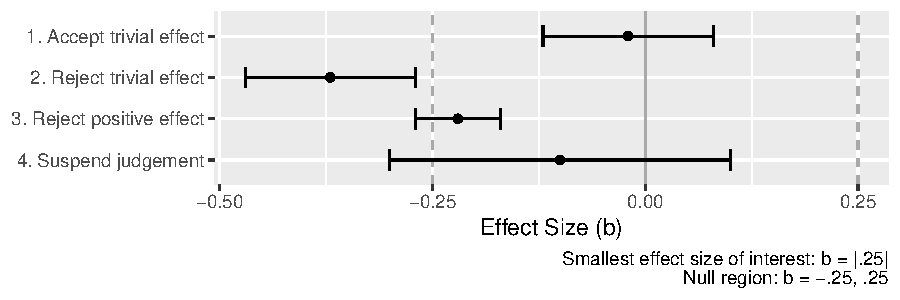
\includegraphics{manuscript_files/figure-latex/sesoi-1.pdf}
\caption{\label{fig:sesoi}Using confidence intervals to test a null region. In this study, a trivial effect of social media use on life satisfaction is defined as ranging from b = -.30 to b = .30. Figure adapted from Dienes (2014).}
\end{figure}

\subsubsection{Causality}\label{causality}

Analyzing causal effects within non-experimental designs requires adopting an internal perspective, focusing on \emph{within-person effects} (Hamaker, 2014).
This entails evaluating how alterations in an individual's media consumption directly impact changes in their own well-being.
Consequently, this study exclusively investigates within-person effects.

An essential strategy for isolating the genuine impact of variables is to \emph{control for confounding factors} that influence both media use and well-being (Rohrer, 2018).
In the context of within-person analysis, this necessitates accounting for time-varying confounders (Rohrer \& Murayama, 2023).
However, a cautious balance must be maintained by not controlling for variables that mediate the relationship (Rohrer, 2018), as their inclusion could distort the assessment of the causal effect.
This study therefore incorporated several control variables (see below), which have demonstrated connections with both social media use and well-being and are likely not mediators (Eger \& Maridal, 2015).

Establishing causality necessitates determining a \emph{plausible temporal interval} (Rohrer \& Murayama, 2023).
For instance, fluctuations in positive and negative affect call for shorter intervals, while the more enduring nature of life satisfaction implies longer intervals (Dienlin \& Johannes, 2020).
In this study, I examine the linkage between changes in social media use and changes in affect within the same week.
Specifically, I investigate if heightened COVID-19-related social media use during a week corresponds with enhanced or diminished affect during that same week.
I consider a longer interval for life satisfaction, examining whether increased COVID-19-related social media use over the course of a week influences one's life satisfaction at the week's end.
Supplementary analyses extend this investigation to observe how media use might affect well-being one or four months later.

\subsubsection{Statistical model}\label{statistical-model}

The hypothesis was analyzed using random effect within-between models (REWB, Bell et al., 2019).
Altogether three models were run, one for each dependent variable.
The data were hierarchical, and responses were separately nested in participants and waves (i.e., participants and waves were implemented as random effects).
Nesting in participants accounts for the within-person design.
Nesting in waves controls for general exogenous developments, such as general decreases in well-being in the population, for example due to lockdown measures.
Thus, there was no need additionally to control for specific phases or measures of the lockdown.
Predictors were modeled as fixed effects.
They included social media communication types and channels, separated into within and between-person factors, as well as stable and varying covariates.
Between-person predictors (which, measuring relations, are not of particular interest in this study, but are reported online) represent how the mean of one respondent differs from the mean of all the other respondents.
The within-person predictors represent how much a person at one specific wave differs from their own mean.
All predictors were included simultaneously in each of the three models.
No collinearity of predictors was observed.

The factorial validity of the scales were tested with confirmatory factor analyses (CFA).
Because Mardia's test showed that the assumption of multivariate normality was violated, I used the more robust Satorra-Bentler scaled and mean-adjusted test statistic (MLM) as estimator.
Mean scores were used for positive and negative affect.
Although imputation has inherent drawbacks, we followed recent recommendations to impute missing data on larger scales (Enders, 2022).
Missing responses were imputed using multiple imputation with predictive mean matching (five iterations, 30 data-sets), including categorical variables.
All variables were imputed except the social media use measures, as they were not collected on each wave.
All variables included in the analyses presented here were used to impute missing data.
For the main analyses, results were pooled across all thirty data-sets.

To contextualize the results, I conducted additional exploratory analyses (see online materials)
I reran the analyses (a) with additional not-preregistered covariates such as trust in media or government, (b) without covariates, (c) with single imputation, and (d) without imputation.

\subsection{Measures}\label{measures}

\subsubsection{Well-being}\label{well-being}

Life satisfaction was measured with the item ``All things considered, how satisfied are you with your life as a whole nowadays?'', which comes from the European Social Survey.
The response options ranged from 0 (\emph{extremely dissatisfied}) to 10 (\emph{extremely satisfied}).

To capture positive affect, respondents were asked how often in the last week they felt (a) calm and relaxed, (b) happy, and (c) full of energy (World Health Organization, 1998).
The response options were 1 (\emph{never}), 2 (\emph{on some days}), 3 (\emph{several times per week}), 4 (\emph{almost every day}), and 5 (\emph{daily}).
The scale showed good factorial fit, \(\chi^2\)(66) = 69.42, \textit{p} = .363, cfi = 1.00, rmsea \textless{} .01, 90\% CI {[}\textless{} .01, .02{]}, srmr = .01.
Reliability was high, \(\omega\) = .85.

For negative affect, respondents were asked how often in the last week they felt (a) lonely, (b) aggravated, (c) so depressed, that nothing could lift you up, (d) very nervous, (e) anxious, and (h) glum and sad (World Health Organization, 1998).
The response options were 1 (\emph{never}), 2 (\emph{on some days}), 3 (\emph{several times per week}), 4 (\emph{almost every day}), and 5 (\emph{daily}).
The scale showed good factorial fit, \(\chi^2\)(471) = 4012.14, \textit{p} \textless{} .001, cfi = .98, rmsea = .07, 90\% CI {[}.07, .08{]}, srmr = .03.
Reliability was high, \(\omega\) = .91.

All three variables were measured on each wave.

\subsubsection{COVID-19 related social media use}\label{covid-19-related-social-media-use}

COVID-19 related social media use focused on communication types was measured with the three dimensions of (a) reading, (b) liking and sharing, and (c) posting.
The items come from Wagner et al. (2018) and were adapted for the context of this study.
The general introductory question was ``How often during the last week have you engaged in the following activities on social media?''.
The three items were ``Reading the posts of others with content on the Coronavirus'', ``When seeing posts on the Coronavirus, I clicked `like', `share' or `retweet'\,'', ``I myself wrote posts on the Coronavirus on social media.''
Answer options were 1 (\emph{several times per day}), 2 (\emph{daily}), 3 (\emph{several times per week}), 4 (\emph{weekly}), 5 (\emph{never}).
The items were inverted for the analyses.

COVID-19 related social media use focused on channels was measured with five variables from Wagner et al. (2018), adapted for this study.
The general introductory question was ``How often in the last week have you followed information related to the Corona-crisis on the following social media?''
The five items were (a) Facebook, (b) Twitter, (c) Instagram, (d) Youtube, and (e) WhatsApp.
Again, the answer options were 1 (\emph{several times per day}), 2 (\emph{daily}), 3 (\emph{several times per week}), 4 (\emph{weekly}), 5 (\emph{never}).
Again, the items were inverted for the analyses.

Social media use was measured for all participants on waves 1, 2, 8, 17, 23, and 28 (see Figure 1).
Freshly recruited respondents always answered all questions on COVID 19-related social media use.
Because new respondents always provided data on media use, it was possible to include these data into the analyses.
Hence, for the main analyses data from all 34 waves were used.

\subsubsection{Control variables}\label{control-variables}

The effects of COVID-19 related social media use were controlled for the following stable variables:
gender (female, male, diverse), age, education (ten options), Austria country of birth (yes/no), Austria parents' country of birth (no parent, one parent, both parents), and household size.
I also controlled for the following varying covariates: five items on current living conditions, including self-reported physical health, whether participants contracted COVID-19 since the last wave, current household income, working in home-office, and overall work hours; nine items measuring use of specific national text-based and video-based news outlets; five items measuring outdoor activities such as exercise or meeting friends; and two more psychological measures including locus of control and disposition to take risks.

\section{Results}\label{results}

\subsection{Descriptive Analyses}\label{descriptive-analyses}

Looking at the variables from a descriptive perspective, aligned with set-point theory we can see that the level of all well-being measures were comparatively stable during data collection (see Figure \ref{fig:fig-descriptives}).
COVID-19 related social media use, however, showed changes.
Reading, sharing and liking COVID-19 related content decreased substantially (almost one scale point from 3 to 2).
Posting about COVID-19 related content stayed the same.
Using Facebook and WhatsApp for COVID-19 related content decreased.
Instagram, YouTube, and Twitter stayed the same.
The general initial decrease could be explained by the fact that the collection of data began at the end of March 2020, hence approximately three months after the pandemic's onset.
After an initial uptick, COVID-19 related social media use might have already been declining at the time.

\begin{figure}
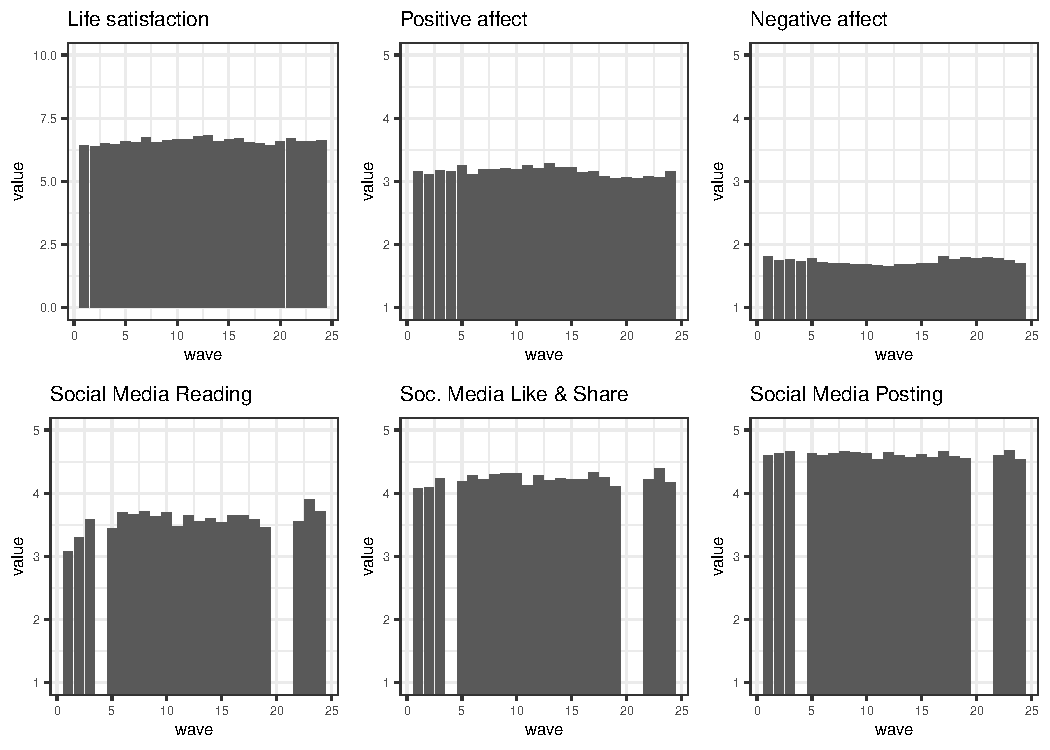
\includegraphics[width=\textwidth]{figures/fig_descriptives} \caption{Well-being and media use across the 34 waves. Note. Values obtained from mixed effect models, with participants and waves as grouping factors and without additional predictors.}\label{fig:fig-descriptives}
\end{figure}

Using the average values across all waves, which provides a stable picture of the general relations, I next looked at the correlations between social media use and well-being (see Figure \ref{fig:fig-correlations}).
In general, people who spend more time engaging with COVID-19 related content on social media reported reduced well-being.
Users who spend more time reading, liking and sharing, and posting COVID-19 related content were less satisfied with their lives.
They also showed slightly less positive affect.
This overall negative picture was even more pronounced for negative affect.
People who engaged more with COVID-19 related content, including all types and channels of communication, reported substantially higher levels of negative affect.
For example, people who were more likely to post COVID-19 content had much higher levels of negative affect (\emph{r} = .61).
Note that these results represent between-person correlations, not causal within-person effects.

\begin{figure}
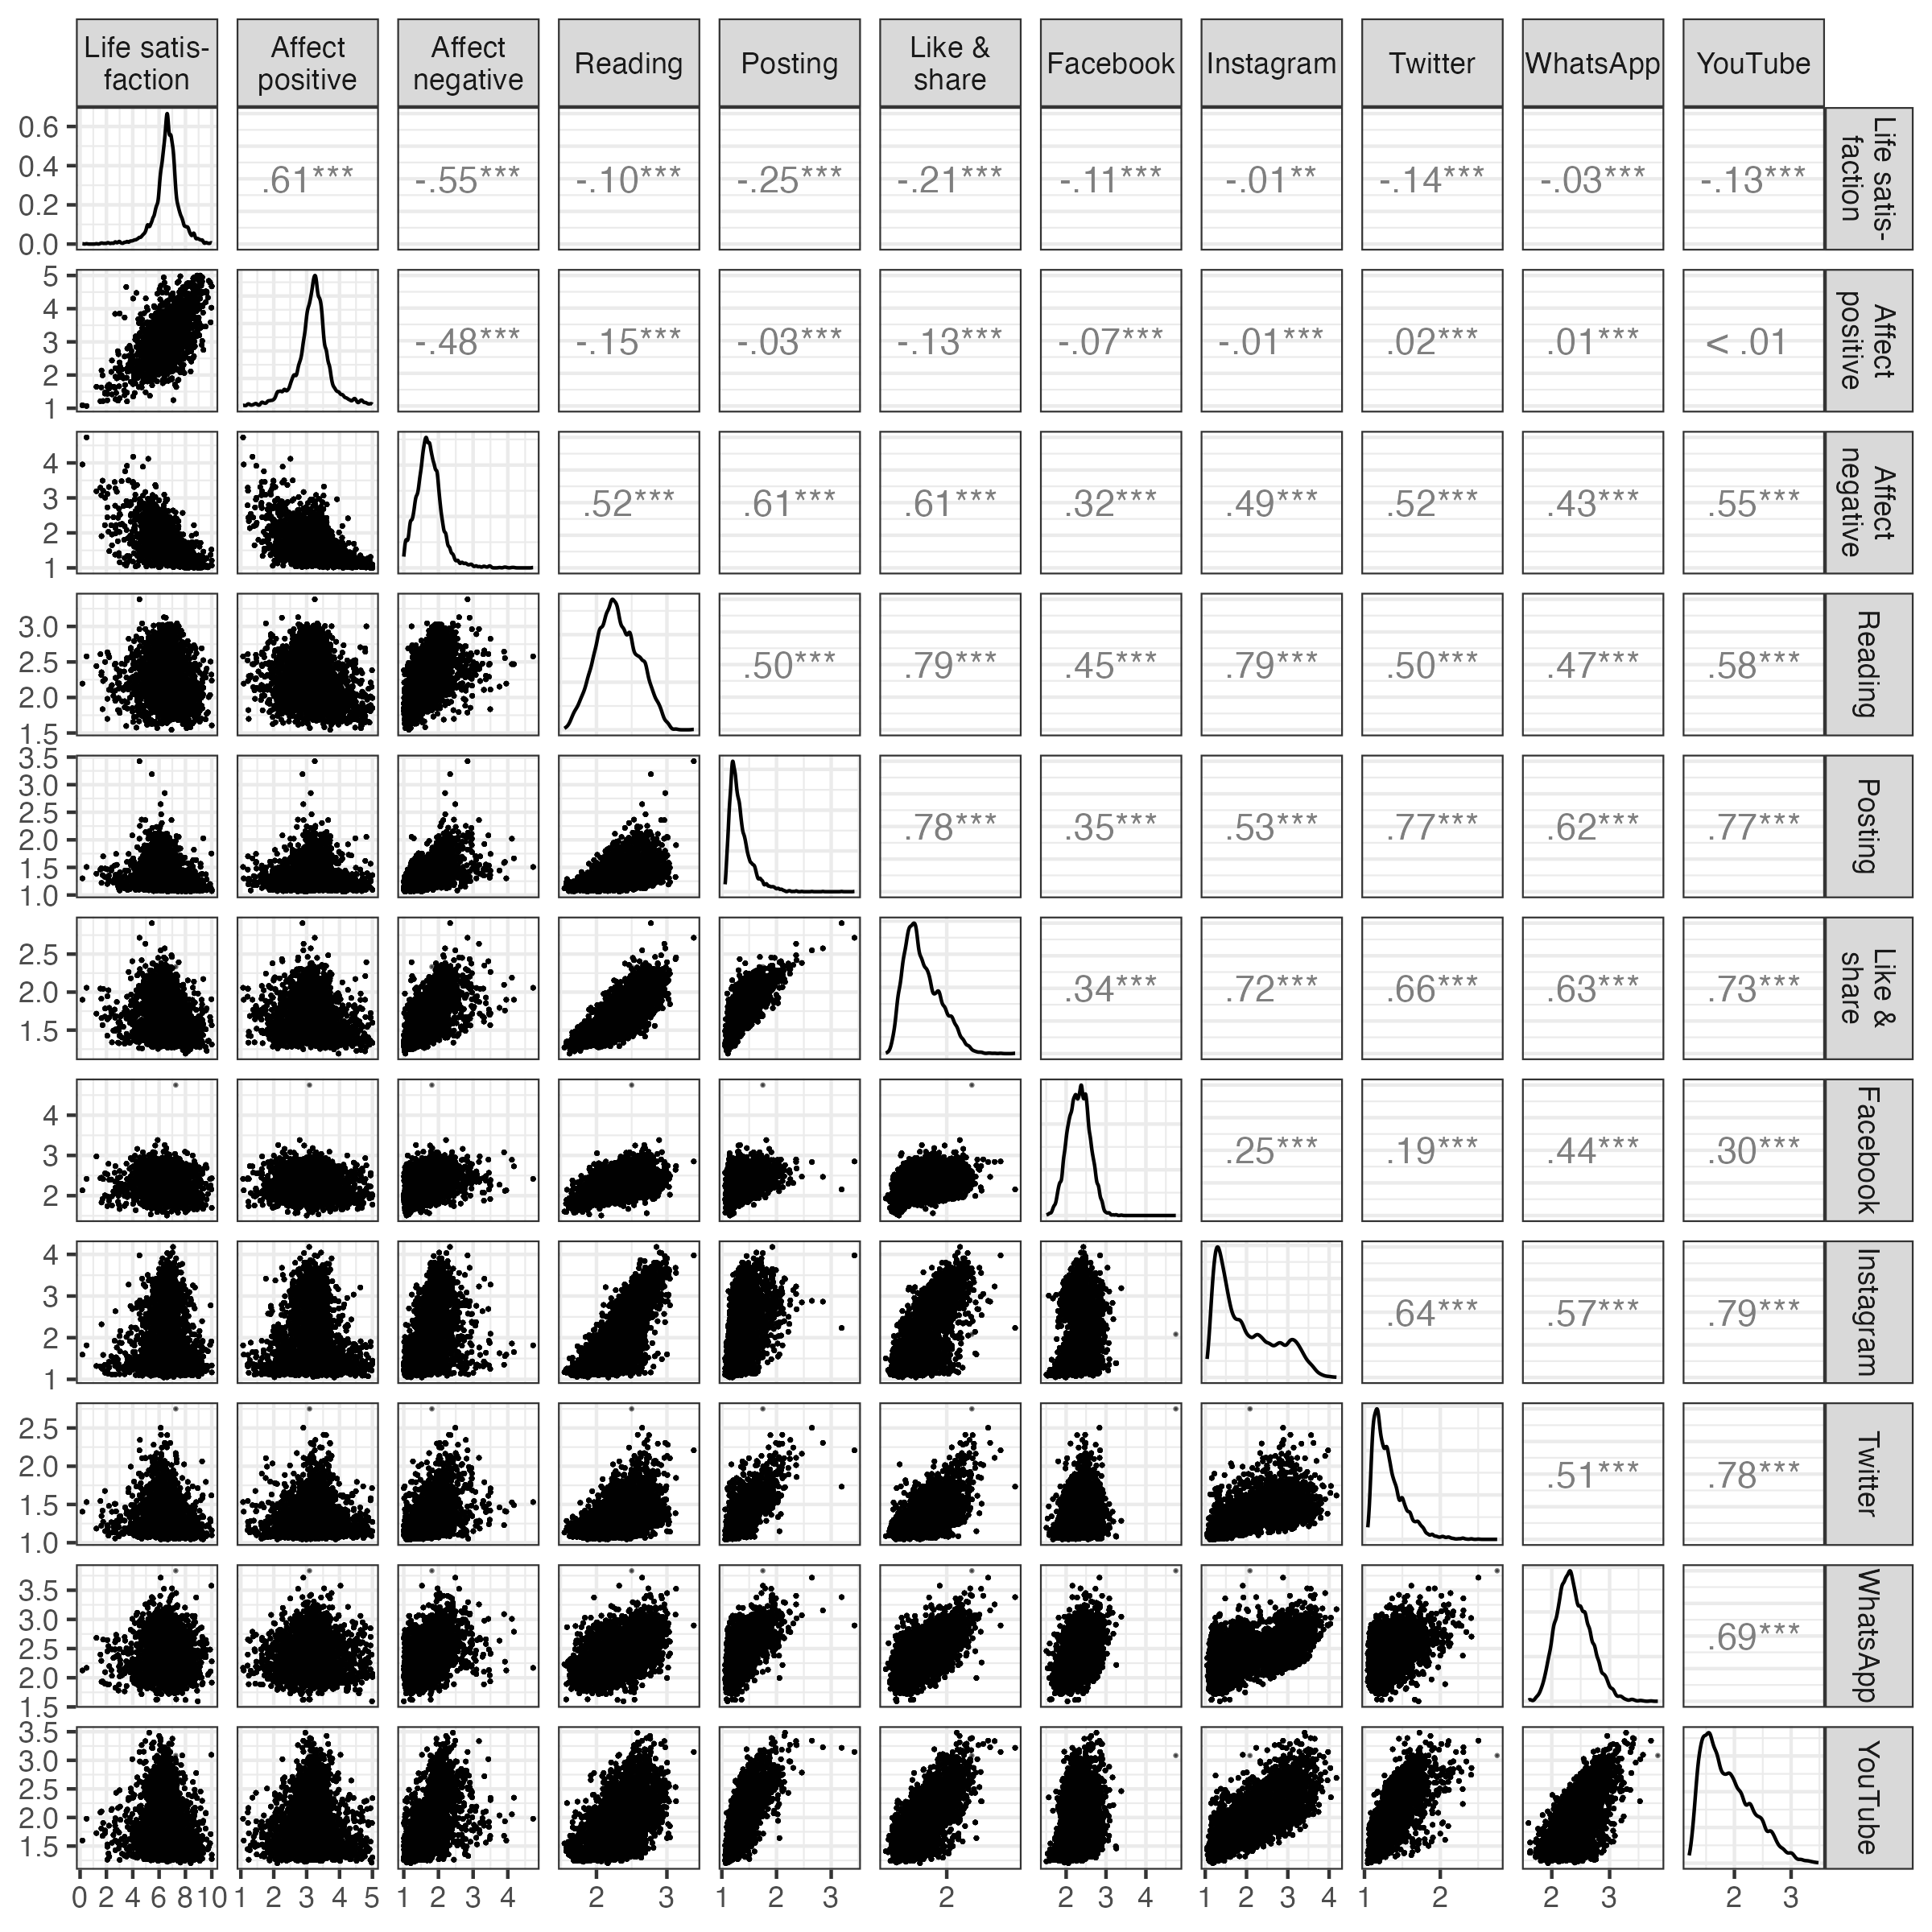
\includegraphics[width=\textwidth]{figures/fig_cor} \caption{Descriptives of the main variables, capturing well-being and social media use with their average values across all waves. Upper triangle: correlation coefficients; diagonal: density plots; lower triangle: scatter plots.}\label{fig:fig-correlations}
\end{figure}

\subsection{Preregistered Analyses}\label{preregistered-analyses}

Regarding the effects of different \emph{communication types} (i.e., reading, sharing, of posting about COVID-19 related content), all within-person effects fell completely within the a-priori defined null region (see Figure \ref{fig:fig-within}).
For example, respondents who used social media more frequently than usual to like or share COVID-19 related content did not show a simultaneous change in life satisfaction (\emph{b} = -0.02 {[}95\% CI -0.06, 0.01{]}).
As a result, the hypothesis of trivial effects was supported for all COVID-19 related types of social media communication.

However, several effects stood out, as statistically they were significantly different from zero.
Users who read more COVID-19 related content than usual reported slightly reduced levels of positive affect (\emph{b} = -0.03 {[}95\% CI -0.05, -0.02{]}).
Users who liked and shared more COVID-19 related content than usual also experienced slightly more negative affect than usual (\emph{b} = 0.05 {[}95\% CI 0.04, 0.07{]}).
Posting COVID-19 related content affected all types of well-being.
Users who wrote more COVID-19 related posts than usual also reported slightly less life satisfaction than usual (\emph{b} = -0.04 {[}95\% CI -0.08, -0.01{]}) and slightly more negative affect than usual (\emph{b} = 0.05 {[}95\% CI 0.04, 0.07{]}).
Interestingly, however, users who wrote more COVID-19 related posts than usual also experienced slightly \emph{higher} levels of positive affect than usual (\emph{b} = 0.02 {[}95\% CI 0.01, 0.04{]}).

Regarding the COVID-19 related use of \emph{social media channels} (i.e., Facebook, Instagram, WhatsApp, YouTube, and Twitter) the results were comparable (see Figure \ref{fig:fig-within}).
Changes in the frequency of using different social media channels to attain information regarding COVID-19 were unrelated to meaningful changes in well-being.
For example, respondents who used Facebook more frequently than usual to learn about COVID-19 did not show a simultaneous change in life satisfaction (\emph{b} -0.01 {[}95\% CI -0.04, 0.02{]}).
In sum, the hypothesis of trivial effects was supported also for the COVID-19 related use of important social media channels.

That said, two effects differed statistically from zero.
Respondents who used Twitter more frequently than usual to attain COVID-19 related content reported slightly higher levels of negative affect than usual (\emph{b} = 0.02 {[}95\% CI 0.01, 0.04{]}).
Likewise, respondents who used YouTube more frequently than usual for COVID-19 related issues reported slightly higher levels of negative affect than usual (\emph{b} = 0.01 {[}95\% CI \textless{} 0.01, 0.02{]}).
However, both effects were still completely inside of the null region, hence likely not large enough to be considered meaningful.

For an overview of all within-person effects, see Figure \ref{fig:fig-within}.

\begin{figure}
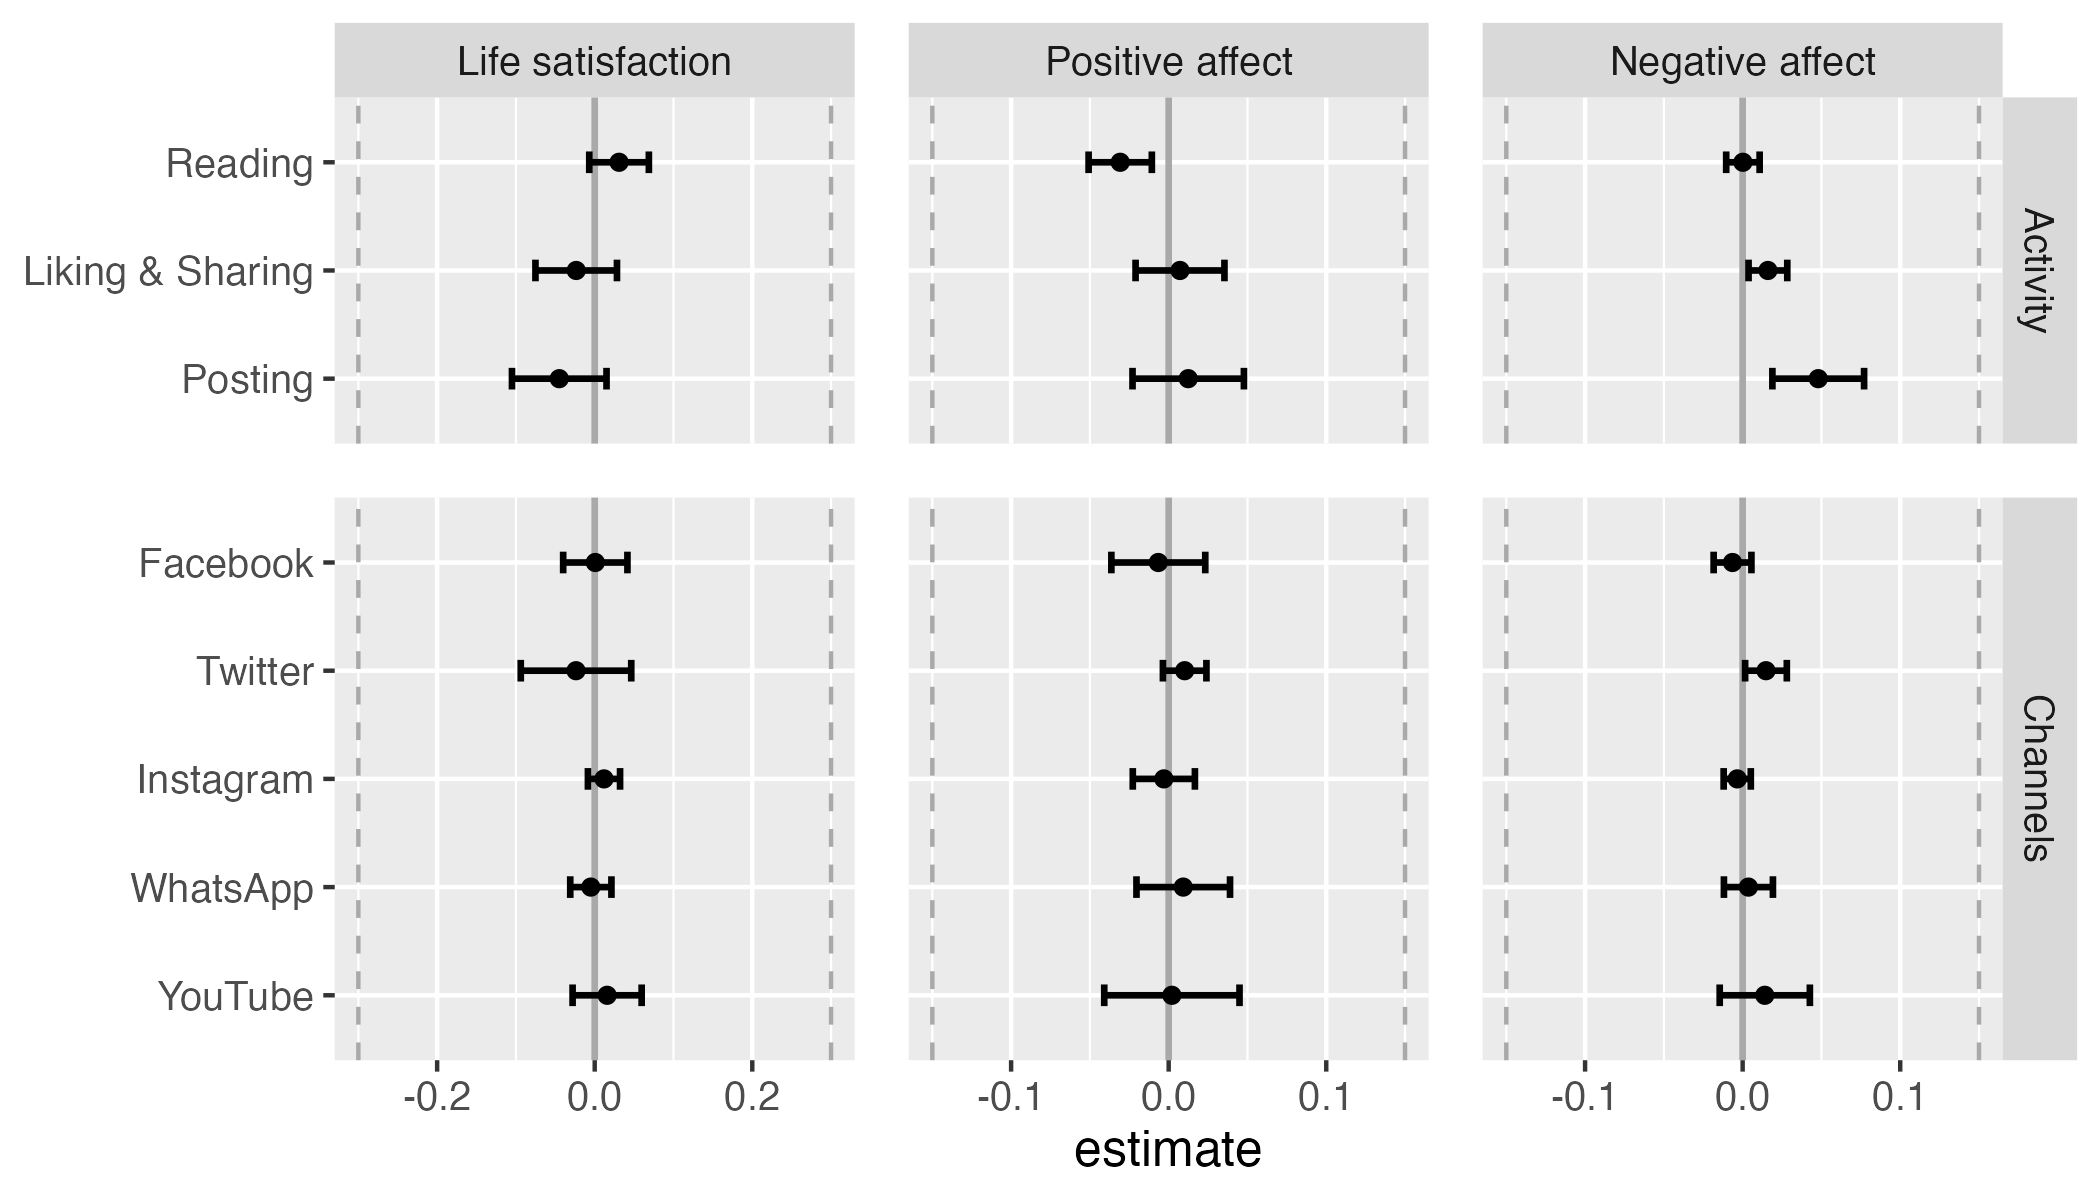
\includegraphics[width=\textwidth]{figures/fig_results_within} \caption{Unstandardized within-person effects of COVID-19 related social media use on well-being. Note. The SESOI was b = |0.30| for life satisfaction and b = |0.15| for affect. Hence, all of the reported effects are not considered large enough to be meaningful.}\label{fig:fig-within}
\end{figure}

\subsection{Exploratory Analyses}\label{exploratory-analyses}

To contextualize the results reported above and to see if the study included any meaningful effects at all, I also looked at the effect sizes of the covariates.
I report the results of the standardized scales, which allows for a better comparison across the differently scaled variables.
As a SESOI, we can build on Cohen's convention that small effects begin at \emph{r} = \textbar.10\textbar.

The results showed that several effects crossed or fell completely outside of the SESOI, and can hence be considered meaningful.
For example, if physical health decreased, this had a meaningful detrimental impact on life satisfaction (\(\beta\) = .19 {[}95\% CI .18, .20{]}), positive affect (\(\beta\) = .18 {[}95\% CI .17, .19{]}), and negative affect (\(\beta\) = -.19 {[}95\% CI -.20, -.18{]}).
Spending more time outside to exercise meaningfully increased positive affect (\(\beta\) = .12 {[}95\% CI .11, .14{]}).
The strongest aspect affecting well-being was internal locus of control.
If people felt more in control of their lives, this strongly increased both life satisfaction (\(\beta\) = .33 {[}95\% CI .31, .35{]}) and
positive affect (\(\beta\) = .28 {[}95\% CI .27, .30{]}),
while decreasing negative affect (\(\beta\) = -.29 {[}95\% CI -.31, -.27{]}).
For an overview, see Figure \ref{fig:fig-control}.

\begin{figure}
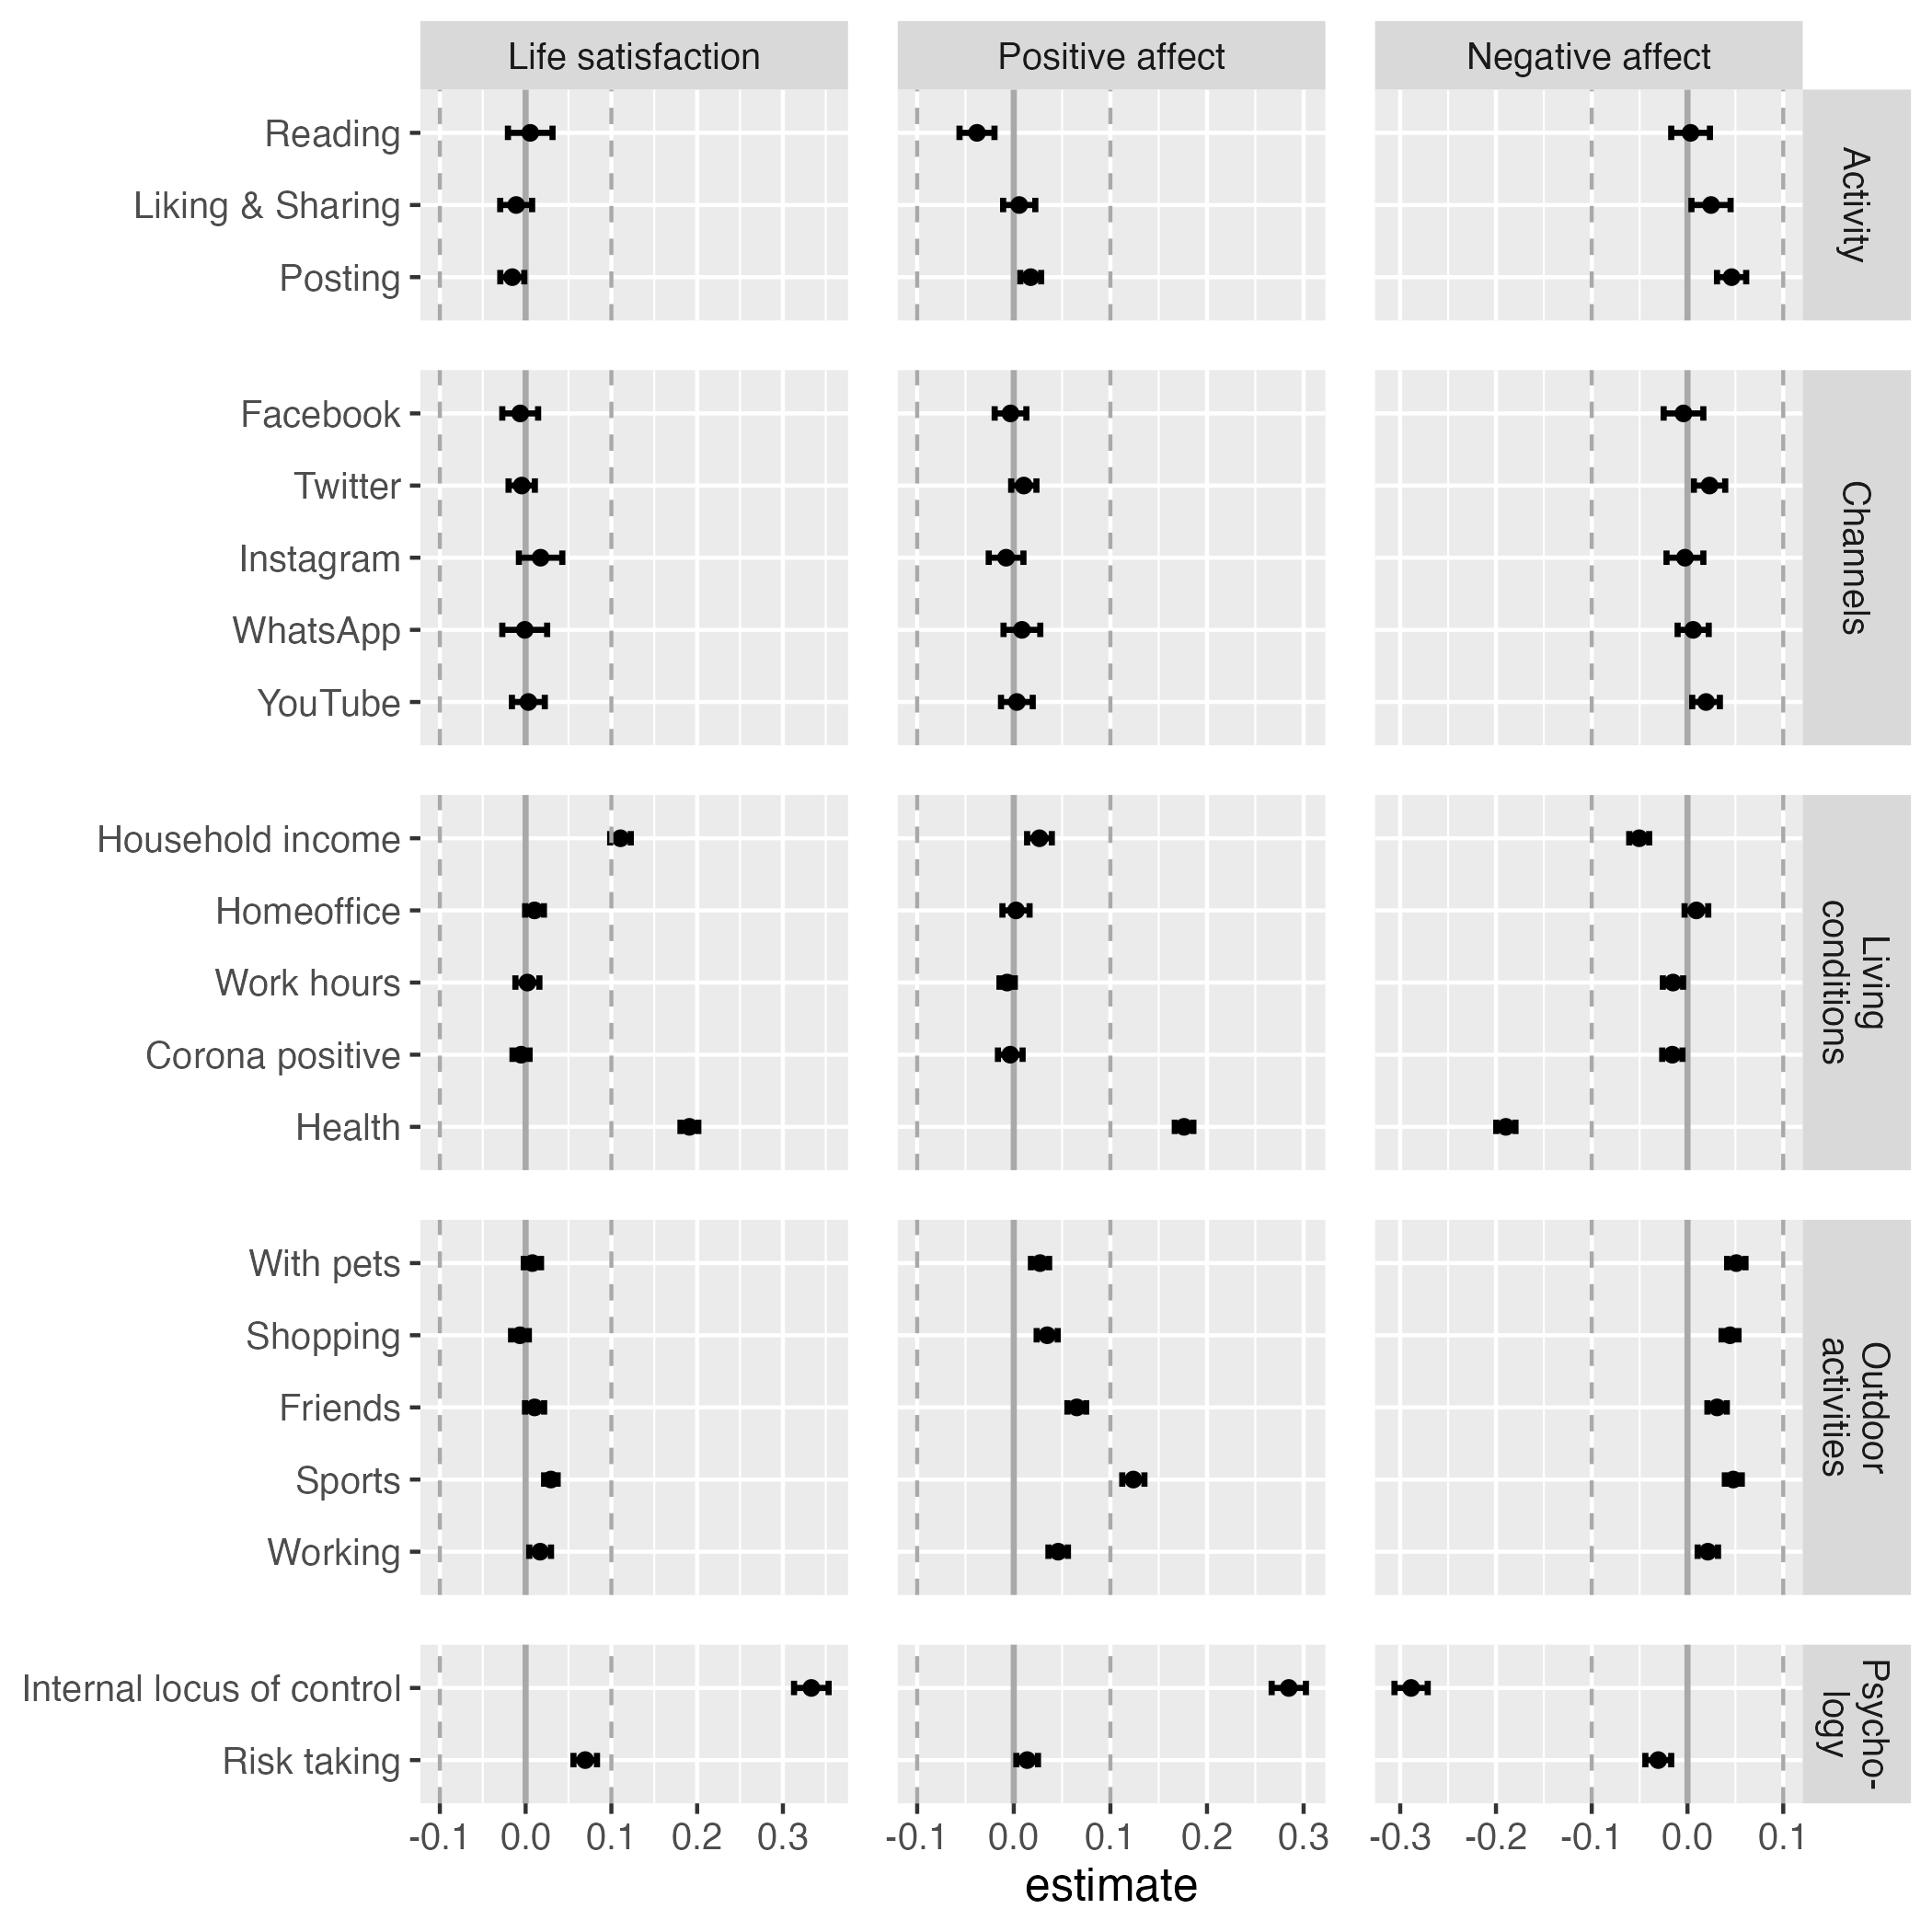
\includegraphics[width=\textwidth]{figures/fig_results_comp_std} \caption{Results of main variables together with covariates to provide context. All variables standardized. SESOI: beta = |.10|}\label{fig:fig-control}
\end{figure}

Because life satisfaction is more stable than affect, the effects of communication might materialize some time later.
I hence also tested the effects across the longer intervals of one month and four months.
Results showed that all effects disappeared.
No effect remained significant, implying that at least in this case in this case effects take place on a shorter interval.

Finally, as suggested by the differential susceptibility of media effects model, media effects can depend on dispositional factors, developmental stages, or cultural norms (Valkenburg \& Peter, 2013), such as gender and age (Orben et al., 2022).
I hence reran the analyses, differentiating effects for boys and girls and for age cohorts.
The results showed that effects did not differ across genders.
The effects also did not depend on age.
However, one effect stood out and was significant.
Compared to the middle age category Generation X, results showed that if users from Generation Z posted more COVID-19 content than usual this lead to significantly more negative affect (\(\beta\) = .04 {[}95\% CI .01, .06{]}).

\section{Discussion}\label{discussion}

This study, based on a representative panel study spanning 34 waves within the Austrian population, investigated the impact of COVID-19-related social media usage on well-being.
The between-person correlations revealed that increased engagement with COVID-19 content on social media was associated with decreased well-being.
For instance, individuals consuming more COVID-19-related content reported slightly lower life satisfaction, somewhat reduced positive affect, and notably elevated negative affect compared to others.

To explore if these between-person correlations translated into within-person effects, it was examined whether within-person changes in media consumption corresponded with within-person changes in well-being.
As expected and aligned with the literature, increased consumption of COVID-19 content did not significantly decrease well-being at a meaningful level.
While several statistically significant effects emerged, their magnitudes were notably small.
For instance, reading more COVID-19 posts than usual slightly decreased positive affect.
Liking and sharing more COVID-19 content than usual were associated with slightly higher negative affect.
Posting more COVID-19 content reduced life satisfaction slightly while elevating both positive and negative affect.
The effects, although statistically significant, fell within a predefined range considered insignificant.

That said, there is no consensus among scholars as to when effects become practically relevant and meaningful.
If we adopt a more liberal and cautious perspective, the study indicates a tendency for COVID-19-related social media usage to impact well-being negatively more frequently than positively.
Notably several statistically significant negative effects were observed, contrasting with a single positive effect.
Hence, although effects were overall very small, the trend was for effects to be negative.

These results align with prior research highlighting that social media usage is rather associated with elevated negative affect but not reduced life satisfaction (Meier \& Reinecke, 2020).
The study suggests that varying communication types and channels warrant separate analyses.
Reading COVID-19 related content slightly reduced positive affect, while liking, sharing, and posting increased negative affect slightly.
Posting COVID-19-related comments increased both negative and positive affect slightly, while it reduced life satisfaction.
Posting COVID-19 content was more negative for Generation Z, potentially reflecting broader negative effects of social media on this generation.
Notably, communication channels exhibited differences.
Twitter and YouTube appeared more negative, whereas Instagram, WhatsApp, and Facebook were neutral.

Several limitations exist. While the study's focus on within-person effects enhances causal understanding, challenges exist related to additional relevant confounding exogenous variables not included here (Rohrer, 2018), correct definition of the SESOI (Anvari \& Lakens, 2021), and exact measurement of media use (Scharkow, 2016).
The measures of social media use did not include interpersonal communication about COVID-19 related content, which might result in more positive outcomes (Frison \& Eggermont, 2015).
The study's results are applicable primarily to Western societies and may not hold true in different cultural contexts.

The study's findings conclude that COVID-19-related social media activity minimally affects well-being, with other factors such as health and physical activity playing more substantial roles.
In light of these minimal effects, concerns over COVID-19-related social media engagement on well-being could not be substantiated.

\newpage

\section{References}\label{references}

\phantomsection\label{refs}
\begin{CSLReferences}{1}{0}
\bibitem[\citeproctext]{ref-anvariUsingAnchorbasedMethods2021}
Anvari, F., \& Lakens, D. (2021). Using anchor-based methods to determine the smallest effect size of interest. \emph{Journal of Experimental Social Psychology}, \emph{96}, 104159. \url{https://doi.org/10.1016/j.jesp.2021.104159}

\bibitem[\citeproctext]{ref-bellFixedRandomEffects2019}
Bell, A., Fairbrother, M., \& Jones, K. (2019). Fixed and random effects models: Making an informed choice. \emph{Quality \& Quantity}, \emph{53}(2), 1051--1074. \url{https://doi.org/10.1007/s11135-018-0802-x}

\bibitem[\citeproctext]{ref-bendauAssociationsCOVID19Related2021}
Bendau, A., Petzold, M. B., Pyrkosch, L., Mascarell Maricic, L., Betzler, F., Rogoll, J., Große, J., Ströhle, A., \& Plag, J. (2021). Associations between {COVID-19} related media consumption and symptoms of anxiety, depression and {COVID-19} related fear in the general population in {Germany}. \emph{European Archives of Psychiatry and Clinical Neuroscience}, \emph{271}(2), 283--291. \url{https://doi.org/10.1007/s00406-020-01171-6}

\bibitem[\citeproctext]{ref-beyensSocialMediaUse2021}
Beyens, I., Pouwels, J. L., van Driel, I. I., Keijsers, L., \& Valkenburg, P. M. (2021). Social media use and adolescents' well-being: {Developing} a typology of person-specific effect patterns. \emph{Communication Research}. \url{https://doi.org/10.1177/00936502211038196}

\bibitem[\citeproctext]{ref-buchananBriefExposureSocial2021}
Buchanan, K., Aknin, L. B., Lotun, S., \& Sandstrom, G. M. (2021). Brief exposure to social media during the {COVID-19} pandemic: {Doom-scrolling} has negative emotional consequences, but kindness-scrolling does not. \emph{PLOS ONE}, \emph{16}(10), e0257728. \url{https://doi.org/10.1371/journal.pone.0257728}

\bibitem[\citeproctext]{ref-carrSocialMediaDefining2015}
Carr, C. T., \& Hayes, R. A. (2015). Social {Media}: {Defining}, {Developing}, and {Divining}. \emph{Atlantic Journal of Communication}, \emph{23}(1), 46--65. \url{https://doi.org/10.1080/15456870.2015.972282}

\bibitem[\citeproctext]{ref-clarkSocialNetworkSites2018}
Clark, J. L., Algoe, S. B., \& Green, M. C. (2018). Social {Network Sites} and {Well-Being}: {The Role} of {Social Connection}. \emph{Current Directions in Psychological Science}, \emph{27}(1), 32--37. \url{https://doi.org/10.1177/0963721417730833}

\bibitem[\citeproctext]{ref-dienerAdvancesOpenQuestions2018}
Diener, E., Lucas, R. E., \& Oishi, S. (2018). Advances and open questions in the science of subjective well-being. \emph{Collabra: Psychology}, \emph{4}(1), 15. \url{https://doi.org/10.1525/collabra.115}

\bibitem[\citeproctext]{ref-dienesUsingBayesGet2014}
Dienes, Z. (2014). Using {Bayes} to get the most out of non-significant results. \emph{Frontiers in Psychology}, \emph{5}. \url{https://doi.org/10.3389/fpsyg.2014.00781}

\bibitem[\citeproctext]{ref-dienlinImpactDigitalTechnology2020}
Dienlin, T., \& Johannes, N. (2020). The impact of digital technology use on adolescent well-being. \emph{Dialogues in Clinical Neuroscience}, \emph{22}(2), 135--142. \url{https://doi.org/doi:10.31887/DCNS.2020.22.2/tdienlin}

\bibitem[\citeproctext]{ref-edenMediaCopingCOVID192020}
Eden, A. L., Johnson, B. K., Reinecke, L., \& Grady, S. M. (2020). Media for coping during {COVID-19} social distancing: {Stress}, anxiety, and psychological well-being. \emph{Frontiers in Psychology}, \emph{11}, 577639. \url{https://doi.org/10.3389/fpsyg.2020.577639}

\bibitem[\citeproctext]{ref-egerStatisticalMetaanalysisWellbeing2015}
Eger, R. J., \& Maridal, J. H. (2015). A statistical meta-analysis of the wellbeing literature. \emph{International Journal of Wellbeing}, \emph{5}(2), 45--74. \url{https://doi.org/10.5502/ijw.v5i2.4}

\bibitem[\citeproctext]{ref-endersAppliedMissingData2022}
Enders, C. K. (2022). \emph{Applied missing data analysis} (Second Edition). The Guilford Press.

\bibitem[\citeproctext]{ref-fanInformationOverloadWellbeing2021}
Fan, J., \& Smith, A. P. (2021). Information overload, wellbeing and {COVID-19}: {A} survey in {China}. \emph{Behavioral Sciences}, \emph{11}(5), 62. \url{https://doi.org/10.3390/bs11050062}

\bibitem[\citeproctext]{ref-frisonExploringRelationshipsDifferent2015}
Frison, E., \& Eggermont, S. (2015). Exploring the relationships between different types of {Facebook} use, perceived online social support, and adolescents' depressed mood. \emph{Social Science Computer Review}, 1--19. \url{https://doi.org/10.1177/0894439314567449}

\bibitem[\citeproctext]{ref-guazziniSecondWaveAnalysis2022}
Guazzini, A., Pesce, A., Marotta, L., \& Duradoni, M. (2022). Through the second wave: {Analysis} of the psychological and perceptive changes in the {Italian} population during the {COVID-19} pandemic. \emph{International Journal of Environmental Research and Public Health}, \emph{19}(3), 1635. \url{https://doi.org/10.3390/ijerph19031635}

\bibitem[\citeproctext]{ref-hallSocialMediaUse2022}
Hall, J. A., \& Liu, D. (2022). Social media use, social displacement, and well-being. \emph{Current Opinion in Psychology}, \emph{46}, 101339. \url{https://doi.org/10.1016/j.copsyc.2022.101339}

\bibitem[\citeproctext]{ref-hamakerWhyResearchersShould2014}
Hamaker, E. L. (2014). Why researchers should think "within-person": {A} paradigmatic rationale. In M. R. Mehl, T. S. Conner, \& M. Csikszentmihalyi (Eds.), \emph{Handbook of research methods for studying daily life} (Paperback ed.). Guilford.

\bibitem[\citeproctext]{ref-huntSocialMediaBased2022}
Hunt, I. de V., Dunn, T., Mahoney, M., Chen, M., Nava, V., \& Linos, E. (2022). A social media-based public health campaign encouraging {COVID-19} vaccination across the {United States}. \emph{American Journal of Public Health}, \emph{112}(9), 1253--1256. \url{https://doi.org/10.2105/AJPH.2022.306934}

\bibitem[\citeproctext]{ref-johnhopkinsuniversityCOVID19Map2023}
John Hopkins University. (2023). {COVID-19 Map}. In \emph{Johns Hopkins Coronavirus Resource Center}. https://coronavirus.jhu.edu/map.html.

\bibitem[\citeproctext]{ref-katzUsesGratificationsResearch1973}
Katz, E., Blumler, J. G., \& Gurevitch, M. (1973). Uses and {Gratifications Research}. \emph{Public Opinion Quarterly}, \emph{37}(4), 509. \url{https://doi.org/10.1086/268109}

\bibitem[\citeproctext]{ref-kittelAustrianCoronaPanel2020}
Kittel, B., Kritzinger, S., Boomgaarden, H., Prainsack, B., Eberl, J.-M., Kalleitner, F., Lebernegg, N. S., Partheymüller, J., Plescia, C., Schiestl, D. W., \& Schlogl, L. (2020). \emph{Austrian {Corona Panel Project} ({SUF} edition)}. AUSSDA. \url{https://doi.org/10.11587/28KQNS}

\bibitem[\citeproctext]{ref-latikkaLonelinessPsychologicalDistress2022}
Latikka, R., Koivula, A., Oksa, R., Savela, N., \& Oksanen, A. (2022). Loneliness and psychological distress before and during the {COVID-19} pandemic: {Relationships} with social media identity bubbles. \emph{Social Science \& Medicine}, \emph{293}, 114674. \url{https://doi.org/10.1016/j.socscimed.2021.114674}

\bibitem[\citeproctext]{ref-liYouTubeSourceInformation2020}
Li, H. O.-Y., Bailey, A., Huynh, D., \& Chan, J. (2020). {YouTube} as a source of information on {COVID-19}: A pandemic of misinformation? \emph{BMJ Global Health}, \emph{5}(5), e002604. \url{https://doi.org/10.1136/bmjgh-2020-002604}

\bibitem[\citeproctext]{ref-marcianoDynamicsAdolescentsSmartphone2022}
Marciano, L., Driver, C. C., Schulz, P. J., \& Camerini, A.-L. (2022). Dynamics of adolescents' smartphone use and well-being are positive but ephemeral. \emph{Scientific Reports}, \emph{12}(1), 1316. \url{https://doi.org/10.1038/s41598-022-05291-y}

\bibitem[\citeproctext]{ref-meierComputermediatedCommunicationSocial2020a}
Meier, A., \& Reinecke, L. (2020). Computer-mediated communication, social media, and mental health: {A} conceptual and empirical meta-review. \emph{Communication Research}, 009365022095822. \url{https://doi.org/10.1177/0093650220958224}

\bibitem[\citeproctext]{ref-normanInterpretationChangesHealthrelated2003}
Norman, G., Sloan, J., \& Wyrwich, K. (2003). Interpretation of changes in health-related quality of life: {The} remarkable universality of half a standard deviation. \emph{Medical Care}, \emph{41}(5), 582--592.

\bibitem[\citeproctext]{ref-orbenWindowsDevelopmentalSensitivity2022}
Orben, A., Przybylski, A. K., Blakemore, S.-J., \& Kievit, R. A. (2022). Windows of developmental sensitivity to social media. \emph{Nature Communications}, \emph{13}(1), 1649. \url{https://doi.org/10.1038/s41467-022-29296-3}

\bibitem[\citeproctext]{ref-pelletierOneSizeDoesn2020}
Pelletier, M. J., Krallman, A., Adams, F. G., \& Hancock, T. (2020). One size doesn't fit all: A uses and gratifications analysis of social media platforms. \emph{Journal of Research in Interactive Marketing}, \emph{14}(2), 269--284. \url{https://doi.org/10.1108/JRIM-10-2019-0159}

\bibitem[\citeproctext]{ref-przybylskiMotivationalEmotionalBehavioral2013}
Przybylski, A. K., Murayama, K., DeHaan, C. R., \& Gladwell, V. (2013). Motivational, emotional, and behavioral correlates of fear of missing out. \emph{Computers in Human Behavior}, \emph{29}(4), 1841--1848. \url{https://doi.org/10.1016/j.chb.2013.02.014}

\bibitem[\citeproctext]{ref-rohrerThinkingClearlyCorrelations2018}
Rohrer, J. M. (2018). Thinking clearly about correlations and causation: {Graphical} causal models for observational data. \emph{Advances in Methods and Practices in Psychological Science}, \emph{24}(2), 251524591774562. \url{https://doi.org/10.1177/2515245917745629}

\bibitem[\citeproctext]{ref-rohrerTheseAreNot2023}
Rohrer, J. M., \& Murayama, K. (2023). These are not the effects you are looking for: {Causality} and the within-/between-persons distinction in longitudinal data analysis. \emph{Advances in Methods and Practices in Psychological Science}, \emph{6}(1), 25152459221140842. \url{https://doi.org/10.1177/25152459221140842}

\bibitem[\citeproctext]{ref-sandstromDoomscrollingCOVIDNews2021}
Sandstrom, G., Buchanan, K., Aknin, L., \& Lotun, S. (2021). Doomscrolling {COVID} news takes an emotional toll -- here's how to make your social media a happier place. In \emph{The Conversation}. http://theconversation.com/doomscrolling-covid-news-takes-an-emotional-toll-heres-how-to-make-your-social-media-a-happier-place-170342.

\bibitem[\citeproctext]{ref-scharkowAccuracySelfreportedInternet2016}
Scharkow, M. (2016). The accuracy of self-reported {Internet} use---{A} validation study using client log data. \emph{Communication Methods and Measures}, \emph{10}(1), 13--27. \url{https://doi.org/10.1080/19312458.2015.1118446}

\bibitem[\citeproctext]{ref-sewallObjectivelyMeasuredDigital2021}
Sewall, C. J. R., Goldstein, T. R., \& Rosen, D. (2021). Objectively measured digital technology use during the {COVID-19} pandemic: {Impact} on depression, anxiety, and suicidal ideation among young adults. \emph{Journal of Affective Disorders}, \emph{288}, 145--147. \url{https://doi.org/10.1016/j.jad.2021.04.008}

\bibitem[\citeproctext]{ref-sharmaDarkEndTunnel2022}
Sharma, B., Lee, S. S., \& Johnson, B. K. (2022). The dark at the end of the tunnel: {Doomscrolling} on social media newsfeeds. \emph{Technology, Mind, and Behavior}, \emph{3}(1). \url{https://doi.org/10.1037/tmb0000059}

\bibitem[\citeproctext]{ref-stainbackCOVID1924News2020}
Stainback, K., Hearne, B. N., \& Trieu, M. M. (2020). {COVID-19} and the 24/7 {News Cycle}: {Does COVID-19 News Exposure Affect Mental Health}? \emph{Socius}, \emph{6}, 2378023120969339. \url{https://doi.org/10.1177/2378023120969339}

\bibitem[\citeproctext]{ref-statistaAverageDailyTime2021}
Statista. (2021). \emph{Average daily time spent on social networks by users in the {United States} from 2018 to 2022}. https://www.statista.com/statistics/1018324/us-users-daily-social-media-minutes/.

\bibitem[\citeproctext]{ref-valkenburgDifferentialSusceptibilityMedia2013}
Valkenburg, P. M., \& Peter, J. (2013). The differential susceptibility to media effects model. \emph{Journal of Communication}, \emph{63}(2), 221--243. \url{https://doi.org/10.1111/jcom.12024}

\bibitem[\citeproctext]{ref-vandenabeeleDigitalWellbeingDynamic2021}
Vanden Abeele, M. M. P. (2021). Digital {Wellbeing} as a {Dynamic Construct}. \emph{Communication Theory}, \emph{31}(4), 932--955. \url{https://doi.org/10.1093/ct/qtaa024}

\bibitem[\citeproctext]{ref-verduynSocialNetworkingSites2022}
Verduyn, P., Gugushvili, N., \& Kross, E. (2022). Do {Social Networking Sites Influence Well-Being}? {The Extended Active-Passive Model}. \emph{Current Directions in Psychological Science}, \emph{31}(1), 62--68. \url{https://doi.org/10.1177/09637214211053637}

\bibitem[\citeproctext]{ref-wagnerAUTNESOnlinePanel2018}
Wagner, M., Aichholzer, J., Eberl, J.-M., Meyer, T. M., Berk, N., Büttner, N., Boomgaarden, H., Kritzinger, S., \& Müller, W. C. (2018). \emph{{AUTNES Online Panel Study} 2017 ({SUF} edition)}. AUSSDA. \url{https://doi.org/10.11587/I7QIYJ}

\bibitem[\citeproctext]{ref-worldhealthorganizationWellbeingMeasuresPrimary1998}
World Health Organization. (1998). \emph{Wellbeing measures in primary health care/{The Depcare Project}}.

\bibitem[\citeproctext]{ref-zillmannMoodManagementCommunication1988}
Zillmann, D. (1988). Mood management through communication choices. \emph{American Behavioral Scientist}, \emph{31}(3), 327340. \url{https://doi.org/10.1177/000276488031003005}

\end{CSLReferences}

\section{Acknowledgements}\label{acknowledgements}

I would like to thank BLINDED for providing valuable feedback on this manuscript.


\end{document}
